\chapter{Theory}\label{c:Theory}

\section{Standard Model}


The Standard Model (SM) of particle physics is a collection of several theories which provide the most accurate theoretical framework for describing all known components of matter and their interactions to date. The model describes three fundamental forces, each mediated by an integer spin particle called a \textit{gauge boson}, that control interactions between the spin-$\frac{1}{2}$ \textit{quarks} and \textit{leptons} that make up matter. The mathematical structure is  based on the symmetry group $SU(3)_c\times SU(2)_L\times U(1)_\gamma$ and is required to be gauge-invariant. The Standard Model does not include gravity; gravity cannot be written in the Quantum Field Theories that describe the Standard Model, and gravitational interactions are significantly weaker than the other fundamental forces (Table \ref{t:tab:boson}). As a result, gravitational interactions are neglected hereafter.

	\subsection{Fermions}

		The full set of spin-$\frac{1}{2}$ \textit{fermions}, described in Tables \ref{t:tab:quark} and \ref{t:tab:lepton}, are the quark and lepton families, which each have three generations. For each distinct particle there is a paired \textit{anti-particle} which is identical aside from opposite charge and \textit{handedness}. The handedness or helicity of a particle refers to the projection of the angular momentum of the particle along the direction of the particle momentum. For a spin $\frac{1}{2}$ particle, the angular momentum component can be aligned along the direction of motion (\textit{positive} or \textit{right-handed} alignment) or opposed to it (\textit{negative} or \textit{left-handed} alignment)).

		Most matter consists of the observable first generation of the up and down quarks and the electron which make up protons and neutrons, along with the unobservable electron neutrino. Both the leptons and the quarks obey Fermi-Dirac statistics. Quarks experience all three fundamental forces, charged leptons interacting via the electromagnetic and weak interactions and neutrinos experiencing only the weak interaction. Neutrinos have a special individual feature in that only left-handed neutrinos and right-handed anti-neutrinos have been observed. This asymmetry violates invariance under the \textit{charge} (C) quantum operation and under the \textit{parity} (P) operation individually, but does preserve CP invariance \cite{martinshaw}.

		{
		\setlength{\extrarowheight}{5pt}
		\begin{table}[ht]
			\caption[Properties of Spin-$\frac{1}{2}$ quarks]{Spin-$\frac{1}{2}$ fermions: quarks $q$ \cite{pdg}. The top quark mass is taken from direct measurements.}
			\label{t:tab:quark}
			\medskip
			\centering
			\begin{tabular}{clcc}\toprule
				Generation & Flavour & Charge / $e$ & Mass / GeV \\\midrule
				1    &     Up $u$      &    +2/3   & $0.0022\ _{-0.0004}^{+0.0006}$\\
	    &     Down $d$    &    -1/3   & $0.0047\ _{-0.0004}^{+0.0005}$\\
		    	2    &     Charm $c$      &    +2/3   & $1.28\pm0.03$\\
		    	&     Strange $s$    &    -1/3   & $0.096\ _{-0.004}^{+0.008}$\\
				3    &     Top $t$  &   +2/3   & $173.1\pm0.6$\\
	    &     Bottom $b$   &   -1/3   & $4.18\ _{-0.03}^{+0.04}$\\\bottomrule
			\end{tabular}\\[5pt]
		\end{table}
		}
		\begin{table}[ht]
			\caption[Properties of Spin-$\frac{1}{2}$ leptons]{Spin-$\frac{1}{2}$ fermions: leptons $l$ \cite{pdg}}
			\label{t:tab:lepton}
			\medskip
			\centering
			\begin{tabular}{clcl}\toprule
				Generation & Flavour & Charge / $e$ & Mass / MeV\\\midrule
				1    &     Electron $e$      &    -1   & $0.5109989461\pm0.0000000031$\\
				&     Electron Neutrino $\nu_e$    &   0  & $<2\times10^{-6}$ \\
				2    &     Muon $\mu$      &    -1   & $105.6583745\pm0.0000024$\\
				&     Muon Neutrino $\nu_\mu$    &    0   & $<2\times10^{-6}$ \\
				3    &     Tau $\tau$  &   -1   & $1776.86\pm0.12$\\
				&     Tau Neutrino $\nu_\tau$   &   0   & $<2\times10^{-6}$ \\\bottomrule
			\end{tabular}\\[5pt]
		\end{table}

		Quarks are always confined into colour singlet \textit{hadrons} bound by the strong interaction, which are either \textit{baryons} ($qqq$) like the \textit{proton} ($uud$) and \textit{neutron} ($ddu$), or \textit{mesons} ($q\bar{q}$) like the positive \textit{pion} ($u\bar{d}$).

	\newpage
	\subsection{Forces}

		All forces arise due the exchange of unobservable virtual particles, gauge bosons, which obey Bose-Einstein statistics. The three fundamental particle interactive forces for the Standard Model are named the strong, weak and electromagnetic interactions, and are mediated by \textit{gluons}, \textit{weak bosons} and \textit{photons} respectively. The gauge bosons are described in more detail in Table \ref{t:tab:boson}.

		\begin{table}[ht]
			\caption[Properties of Spin-$1$ gauge bosons]{Spin-1 gauge bosons. The strength of the interaction is typically stated in terms of $\alpha$, a dimensionless constant proportional to the matrix element for the virtual particle exchange for each interaction. The weak interaction is intrinsically stronger than the EM interaction, but the mass of the weak bosons limits the range to extremely short distances.  The strength of gravity is $\sim10^{-39}$ hence it is neglected. \cite{pdg}}
			\label{t:tab:boson}
			\medskip
			\centering
			\begin{tabular}{clclc}\toprule
				Interaction & Particle & Charge / $e$ & Mass / GeV & Strength ($\alpha$) \\\midrule
				Strong    &     Gluon $g$      & 0 & 0 & $\sim1$\\
				Weak (Charged Current)&     $W^+$    &    1   & $80.385\pm0.015$ & \\
				&     $W^-$    &    -1   & $80.385\pm0.015$ & $10^{-6}$ \\
				Weak (Neutral Current)&     $Z$   &    0   & $91.1876\pm0.0021$ & \\
				Electromagnetic (EM)   &     Photon $\gamma$  &  $<1\times10^{-35}$   & $<1\times10^{-27}$ & $\frac{1}{137}$\\\bottomrule
			\end{tabular}\\[5pt]
		\end{table}

		Along with gauge bosons acting as force carriers for interactions, most gauge bosons have a degree of self-coupling which leads to self-interactions. The gluon couples with particles that contain-colour charge, but as the gluon itself possesses a colour charge, gluons may interact with other gluons in exchange processes similar to the exchange of a force carrier between two interacting particles. This self-interacting behaviour is also seen in the $W$ and $Z$ bosons as they couple to the weak charge they carry, but no self-interactions are observed for the photon as it does not carry electromagnetic charge \cite{martinshaw}.

		\subsubsection{Quantum Chromodynamics}

		Quantum Chromodynamics (QCD) is the theory of the strong interaction mediated by the gluon which couples to colour charge. It corresponds to the $SU(3)_c$ symmetry group of the overall Standard Model. The strong interaction conserves energy, momentum, angular momentum and colour charge. Only quarks and gluons themselves possess colour charge, so quarks are the only fermions to feel the strong interaction. As highlighted above, this also means gluons are capable of self interaction, which leads to two distinct properties of the string interaction: \textit{colour confinement} and \textit{asymptotic freedom}.

		Colour confinement is the requirement that observable states have net zero colour charge. This means gluons, like quarks, are only observed in bound states. Asymptotic freedom describes how the interaction gets weaker at short distances, and means that at close distances, such as quark-quark scattering, the interaction normally proceeds through a lowest-order single gluon exchange interaction. The converse of this is that the force increases significantly as the interaction distance increases and higher-order Feynmann interaction diagrams become significant \cite{martinshaw}.

		\subsubsection{Electroweak Unification}

		Electroweak Unification (EW) is the expression of the electromagnetic interaction and the weak interaction as separate manifestations of a combined electroweak force in the Glashow-Weinberg-Salam model \cite{gws-g, gws-w, gws-s}, which corresponds to the $SU(2)_L\times U(1)_Y$ symmetry group. Quantum Electrodynamics (QED) describes the macroscopically observable $U(1)$ electromagnetic force  with the photon as the mediating boson, and any interaction conserves energy, momentum, parity and charge and, additionally, never changes particle type through the interaction. The $SU(2)$ weak interaction is mediated by the charged current vector bosons $W^+$, $W^-$ and the neutral current vector boson $Z$, which have large masses that limit the weak interaction to very short distances. The charged current interaction is capable of changing the flavour of a particle and also of violating parity in an interaction.

		The weak interaction by itself was observed to diverge from observation at high energies, leading to the introduction of the unified theory. The combined $SU(2)_L\times U(1)_Y$ group produces four gauge bosons which mix to produce the more recognisable $\gamma$, $W^+$, $W^-$ and $Z$ bosons. This weak interaction couples to weak isospin charge, which is an analogous quantity to the colour charge of QCD. As the weak bosons carry weak isospin charge themselves, self coupling of the weak bosons is permitted, but is forbidden for the photon as it does not carry electric charge. The weak interaction has been experimentally observed to violate parity conservation \cite{parityviolation, martinshaw}.

		While the weak interaction acts on both quarks and leptons, weak interaction in the quark sector is affected by \textit{quark mixing}. In this construction, the quark mass eigenstates $q$ participate in weak interactions via the weak eigenstates $q^\prime$ formed from linear combinations of the $q$ states \cite{martinshaw}. The observable result of this quark mixing is that different flavour changing interactions have different strengths.

		\newpage
		The coupling relationships of the weak and mass eigenstates is described by the unitary Cabbibo-Kobayashi-Makasawa  matrix $V_{CKM}$ \cite{ckm-c, ckm-km}

		\begin{equation}
		\begin{pmatrix}
		d^\prime \\
		s^\prime\\
		b^\prime \\
		\end{pmatrix}
		 = \begin{pmatrix}
		V_{ud} & V_{us} & V_{ub} \\
		V_{cd} & V_{cs} & V_{cb} \\
		V_{td} & V_{ts} & V_{tb} \\
		\end{pmatrix}
	    \begin{pmatrix}
	    d \\
	    s\\
	    b \\
	    \end{pmatrix}
		\end{equation}

		shown here transforming between the two sets of eigenstates $q$ and $q^\prime$. The CKM matrix elements $V_{\alpha\Beta}$ of $V_{CKM}$ describe the relative couplings of the eigenstates, and are parametrised in terms of three mixing angles and one complex phase \cite{ckm-km, ckmparam}.

	\subsection{Spontaneous Symmetry Breaking: The Higgs Boson}
	\label{t:symbreak}

	The gauge field theories used for the QCD and EW models when unaltered require massless gauge bosons to preserve gauge invariance. This is satisfactory for the gluon and photon, but a separate theory is required to explain the mass of the $W^\pm$ and $Z$ bosons. The \textit{Higgs mechanism} proposed a method for particles to acquire mass by coupling to the spin-$0$ \textit{Higgs} field via the Higgs boson \cite{gauge-boson-mass, higgs-1, higgs-2}. This process as proposed is an example of a \textit{spontaneous symmetry breaking} process, where the gauge invariance of the interaction is preserved but the ground state breaks the invariance.

	The Higgs Mechanism proposed introducing a complex doublet of scalar fields $\phi$ that interact with the $W^\pm$ and $Z$ fields. In the Lagrangian formulation this results in a term akin to a mass term ($\propto\psi^2$) which effectively links that mass of the bosons to their coupling with this scalar field. This field self-interacts to produce a potential energy $V(\phi)$ given by
	 \begin{equation}
		 V(\phi) = \mu^2\phi^2 + \lambda\phi^4
	 \end{equation}

	 	resulting in an equilibrium point ($\phi=0$) that respects the symmetry but is inherently unstable, with an infinite set of degenerate non-zero minima. This minima, the lowest energy level vacuum state, occurs at $|\phi^2|=\nu^2=\frac{-\mu^2}{2\lambda}$ where the symmetry is \textit{spontaneously} broken. This field, in an analogous fashion to the other quantum fields of the Standard Model, can produce particles from excitations which form the physical \textit{Higgs Scalar Boson} $H$.

	 Confirmation of the Higgs boson as part of the Standard Model was only achieved relatively recently \cite{higgs-atlas, higgs-cms}, where a spin-$0$ boson consistent with the Standard Model Higgs boson was observed by the ATLAS and CMS experiments at the LHC. Section \ref{t:higgs} covers in more detail the production and behaviour of the Higgs boson in collider experiments.


\section{Physics of \textit{pp} Collisions}

	\subsection{$pp$ Collisions}
	\label{t:ppc}
	Recent experimental efforts to probe the Standard Model have focused on high-energy collider experiments, where beams of particles with equal energy are collided head on within detector volumes.  For proton-proton ($pp$) collisions, matters are complicated as the colliding protons are composite particles, which at high energy consist of the three \textit{valence} quarks and a sea of virtual quarks and gluons. Collectively these constituents are referred to as \textit{partons}, where each parton carries a fraction of the overall hadron momentum, and the interaction in the $pp$ collision consists of elastic scattering between these partons. At a given energy scale $Q^2$, the probability that a parton $i$ carries a fraction $x_i$ of the overall momentum is described by the parton distribution function (PDF) $f_i(x, Q^2$). These PDFs cannot be calculated from QCD but can be determined from experimental measurements, and collections of PDFs have been assembled from the leading collider experiments \cite{hardinteractions, pdfs}.

	In any particle interaction, the probability of a particular reaction occurring is in proportion to the cross-section of the reaction. The cross-section for a short range, hard parton-parton collision is given by $\hat{\sigma}(Q^2)$, where scattering energy scale $Q^2 = x_1x_2E^2_{cm}$ in the parton-parton centre-of-mass frame where $E_{cm}$ is the energy in the centre-of-mass frame. To compute the cross-section $\sigma$ for some hard process $pp\rightarrow X$, all possible combinations of incoming partons must be summed over and the momentum fractions integrated over while accounting for the PDFs,
	\begin{equation}
	\label{eq:hard}
	\sigma_{pp\rightarrow X} = \sum_{i, j} \int dx_1dx_2f_i(x_1, Q^2)f_j(x_2, Q^2)\hat{\sigma}_{ij\rightarrow X}(Q^2)
	\end{equation}

	where as above $x_i$ are the momentum fractions and $f_i$ the PDFs \cite{hardinteractions}. The PDFs used in these calculations contain series expansion terms, which as a construction is referred to as perturbation theory. This allows truncation of the series exapnsion to the first few terms, which starts with using just a single term for leading-order (LO) calculations, adding a second for next-to-leading-order (NLO) and continues onwards beyond next-to-next-to-leading-order (NNLO)\cite{hardinteractions}.
	\subsection{Geometry}
	\label{t:geometry}

	The high energy protons used in collisions are relativistic in nature, and as the momenta of the colliding partons are not guaranteed to be equal and opposing there is always an unknown element of longitudinal boosting in $pp$ collisions. As a consequence, use of light-cone coordinates and some definitions of convenient quanties can be of benefit to $pp$ collision analyses \cite{lightcone-all-that}.

	Typically the  particle kinematics are defined by transverse momentum \pt and rapidity~$y$. Rapidity is defined by
	\begin{equation}
	y = \frac{1}{2}\ln\frac{E+p_z}{E- p_z}
	\end{equation}

	where $E$ is the energy of a particle and $p_z$ is the momentum component along the beam axis $z$. This rapidity $y$ transforms additively to boosts along the $z$ axis, so any rapidity difference between two objects is invariant to such boosts. For cases where the mass of a particle is negligible (highly relativistic particles) the rapidity can be related to the  pseudo-rapidity $\eta$, defined as
	\begin{equation}
	\eta = -\ln\tan\frac{\theta}{2}
	\end{equation}
	where $\theta$ is the polar angle. The distance between two objects within the detector is commonly expressed in the ($\eta$, $\phi$) space rather than absolute, with this separation being given by $\Delta R = \sqrt{(\Delta\eta)^2 + (\Delta\phi)^2}$.

	\subsection{$pp$ Event Simulations}}

	A $pp$ collision is a complex event which results in a significant number ($\mathcal{O}(1000)$) of final state particles, each of which interact and evolve over the timescale of an event. This progression of the collision event can be broken down into distinct stages of behaviour of the produced particles: the \textit{hard process}, \textit{parton shower}, \textit{hadronisation}, \textit{unstable particle decays} and \textit{underlying event} \cite{monte-carlo}.

	This breakdown is key to the simulation of $pp$ collisions using Monte-Carlo event generators, the use of which is critical in current high energy physics research. Monte-Carlo simulations of collisions are used to predict and prepare for real data-taking experiments, obtain control datasets of particular particle interactions and act as controls to optimise analysis tools. The breakdown of the interaction into distinct stages has allowed specialised software to be produced for each step, which makes use of a characteristic scale and certain safe approximations for the step to provide reliable predictions, while reducing the computational demands of the simulation \cite{monte-carlo}.

	There is a broad selection of software tools for evaluating $pp$ collisions, from general purpose simulations like \textsc{Pythia}\cite{pythia} or \textsc{Sherpa}\cite{sherpa} which are used to evaluate the complete process, to more specific tools like \textsc{Powheg}\cite{powheg} which is used to produce hard scatter events with NLO matrix elements. Most software packages make use of the chain of generation for an event outlined previously, and modern analyses will make use of multiple generators interfaced together to compute different steps with improved accuracy.

		\subsubsection{Hard Process}

			The first stage of a $pp$ collision and the first step of a simulation, the hard scatter refers to highest momentum transfer process in the event between coloured particles, and forms the core of the event. This details the interaction of partons entering the event and those outgoing partons resulting from the process. In simulation the probability distribution of the partons is calculated from perturbation theory to the desired accuracy (LO, NLO etc) using the PDFs of the constituents as covered by equation \ref{eq:hard} in Section \ref{t:ppc}.

		\subsubsection{Parton Shower}

			While the hard scatter interaction in a collision is relatively straightforward, the overall behaviour of the partons is much more complex as they progress through the event. The incoming and outgoing partons from the hard scatter radiate additional  particles during the event \cite{martinshaw, monte-carlo}.
			The Bremsstrahlung  radiation of photons by scattered electric charges is well described by QED, and the analogous radiation of gluons by scattered colour charges as explained by QCD produces additional partons within the interaction. However, as the gluons produced by QCD scattering themselves carry colour charge, there is extending showering of gluons producing gluons, resulting in the phase space of the interaction being filled with a sea of soft gluons. In addition to the self interactions, quark and gluon processes, $g\rightarrow q\bar{q}$ and $q\rightarrow g\bar{g}$, occur. These radiative processes make up the parton shower stage of the event simulation \cite{monte-carlo}.

			The evolution of these parton showers is evaluated in Monte-Carlo simulations using a step-by-step iterative process, on the scale of momentum transfer in the interaction. This process is started at the hard scatter and evolved through the interaction with decreasing momentum scale until the point at which perturbation theory breaks down, necessitating a different evaluation method \cite{monte-carlo}.

		\subsubsection{Hadronisation}
		\label{t:hadronisation}

			The breakdown of perturbation theory at low momentum scales implies the strong force coupling is very large, and observable colourless hadrons are formed from the coloured partons using hadronisation models in order to extend the simulation. These hadrons are the physical final state particles observed in the detector, which exist due to the colour confinement of the quarks and gluons. Within a particle detector collimated \textit{jets} of hadrons are observed rather than individual hadrons. The parton shower process produces large numbers of gluons and quarks moving out in a collimated stream from the interaction. Partons and gluons are not the final state particles and cannot propagate freely, so at this point hadronisation occurs to collect the partons into the final state particles \cite{monte-carlo}.

			In simulation this step involves collecting the partons produced in the parton shower into hadrons, and is typically evaluated using either a String model \cite{stringmodel} or a Cluster model \cite{clustermodel, monte-carlo}. These steps are models, and not calculations as to how the partons combine, as such calculations are prohibited by the breakdown of perturbation theory. The models themselves were produced by tuning the simulations to data from past experiments like the Large Electron-Positron collider previously operational at thr Conseil Europ\'{e}an pour la Recherche Nucl\'{e}aire \cite{tunes}.

		\subsubsection{Unstable Particle Decays}

			The final stage of the evolution of the parton shower considers the hadrons produced during the shower. These hadrons may not be stable particles but could be resonances that go on to decay within the detector to produce the more stable hadrons observed in the data. Most modern simulation software models these decays, but the exact specification of the decay tables and channels has a significant impact on the final state of the simulation \cite{monte-carlo}.

		\subsubsection{Underlying Event}
		\label{t:underlying}

			While the hard scatter and subsequent parton shower results from the highest momentum interaction of the $pp$ collision, the remnants of the proton not involved in this will continue to interact with each other. This produces additional soft hadrons that fill the interaction environment, overlapping with the products of the hard scatter interaction.

			The dominant model for simulation of the underlying event is a perturbative model, where the other components of the event undergo additional discrete hard scatter interactions and corresponding parton showers, which are simulated in an corresponding fashion to the core scattering.



\section{The Higgs Boson}
\label{t:higgs}

	Detecting the Standard Model Higgs boson is strongly dependent on the predominant production and decay channels for the Higgs boson. In this section, the relevant production and decay channels at the Large Hadron Collider (LHC) will be discussed.

	\subsection{Higgs Production}

		While there are many various methods for production of a Higgs boson, at the LHC the cross section is dominated by gluon-gluon fusion (\ggF) as shown in Figure \ref{fig:higgsproductionCS}, with the second largest cross-section arising from Vector Boson Fusion (VBF, Section \ref{t:VBF}). Other significant production processes are the associated production with a weak boson ($WH/ZH$, Higgs-Strahlung) production modes and associated production with top quarks ($ttH$) \cite{LHCHiggsCS}. The lowest order Feynmann diagrams for these processes are shown in Figure \ref{fig:higgsproddiag}.

			\begin{figure}[h]
				\centering
					\begin{minipage}[h]{0.4\linewidth}
						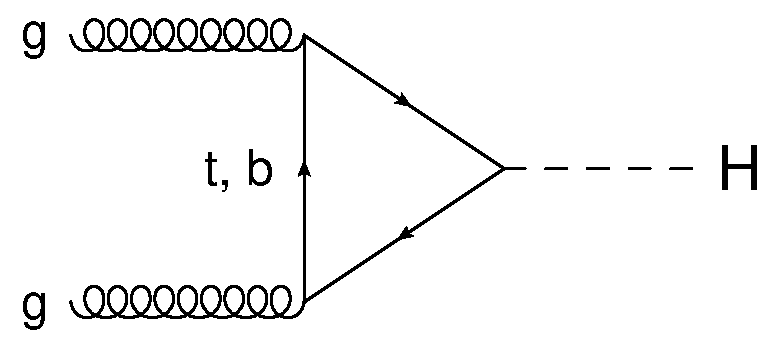
\includegraphics[width=1\linewidth]{T/FIGS/ggF}
					\end{minipage}
					\quad\quad
					\begin{minipage}[h]{0.4\linewidth}
						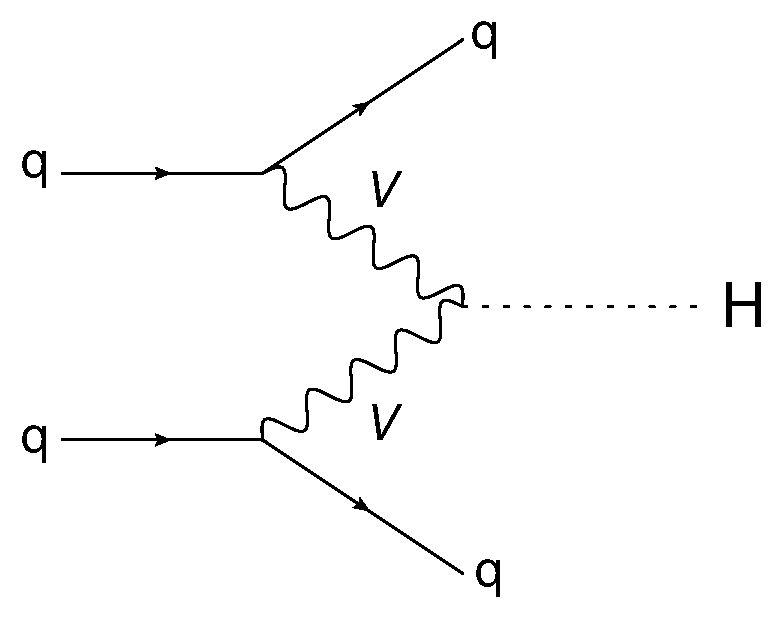
\includegraphics[width=1\linewidth]{T/FIGS/vbf}
					\end{minipage}
					\begin{minipage}[h]{0.4\linewidth}
						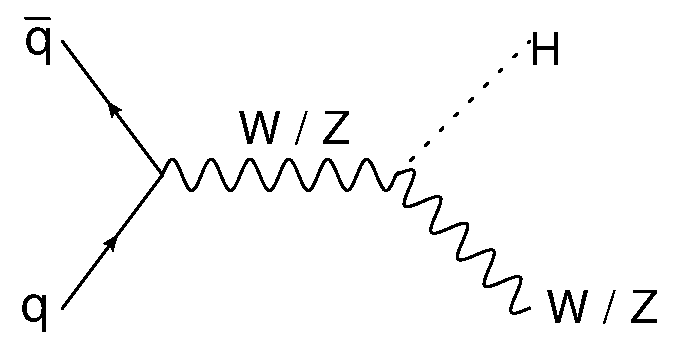
\includegraphics[width=1\linewidth]{T/FIGS/whzh}
					\end{minipage}
					\quad\quad
					\begin{minipage}[h]{0.4\linewidth}
						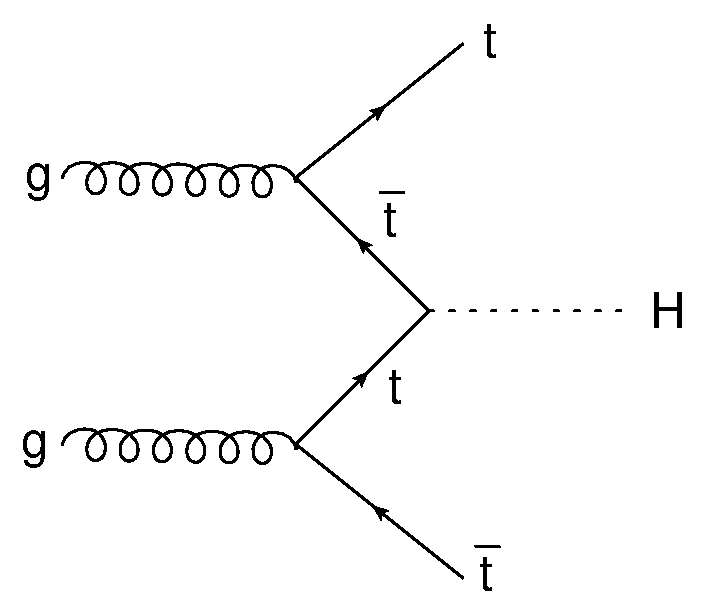
\includegraphics[width=1\linewidth]{T/FIGS/tth}
					\end{minipage}
				\caption[Feynmann diagrams of lowest order Higgs production processes]{Lowest order Feynmann diagrams for gluon-gluon fusion (\ggF), vector boson fusion (VBF), $W/Z$ associated production ($WH/ZH$ or $VH$) and top anti-top associated production ($t\bar{t}H$) \cite{higgsproduction}.}
				\label{fig:higgsproddiag}
			\end{figure}

			\begin{figure}[h]
				\centering
				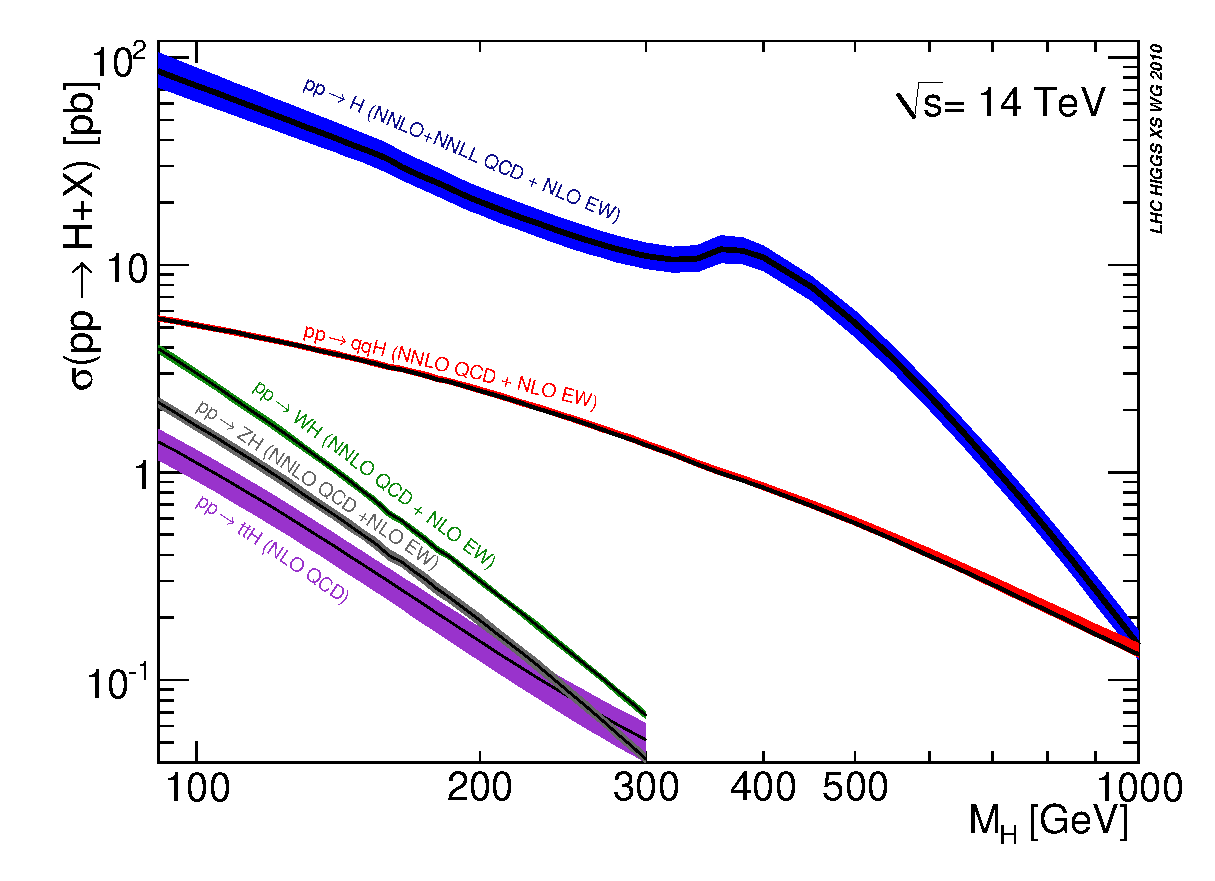
\includegraphics[width=0.7\linewidth]{T/FIGS/YRHXS_Summary_fig3}
				\caption[Higgs production cross section as a function of Higgs mass at a $\sqrt{s}=14$TeV]{SM Higgs Production cross section for $\sqrt{s}=14$ TeV. $\,pp\rightarrow H$ corresponds to gluon-gluon fusion production , $pp\rightarrow qqH$ vector boson fusion, $pp\rightarrow WH$ and $pp\rightarrow ZH$ to $W/Z$ associated production and  $pp\rightarrow ttH$ refers to top anti-top associated production.  \cite{LHCHiggsCS}}
				\label{fig:higgsproductionCS}
			\end{figure}


		The dominant production mechanism for the Higgs boson in hadron colliders is the \ggF\, production via an intermediate quark loop \cite{higgsproduction}. The dynamics of this mechanism are controlled by strong interactions, thus calculations of QCD corrections are necessary for any accurate predictions, and have been computed up from next-to-leading order (NLO) to N$^3$LO for the \ggF\ process in recent years, along with the inclusion of Electro-Weak corrections in the cross-section calculations \cite{LHCHiggsCS}. The \ggf\ production has a cross-section that is between one and two orders of magnitude larger than the other production channels as shown in Figure \ref{fig:higgsproductionCS}. The second largest cross section is that for vector boson fusion, which has a well defined experimental signature due to the two remnant jets produced along with the Higgs boson, and has a well defined NLO cross-section with small QCD corrections \cite{higgssearch}.

		The two other principal production modes at the LHC, the Higgs-strahlung associated $W/Z$ production and associated production with a top quark pair, have very small cross-sections compared to the \ggF\ and VBF production modes. While Higgs searches for these channels must work around the small event rate by using final states with a clear signature, analysis of these channels is possible \cite{higgssearch, tth}.

	\subsection{Higgs Decay}

		The branching ratios for decays of the Higgs boson in the Standard Model have been calculated according to the theoretical framework of the Standard Model \cite{HDECAY}. As is to be expected, the relative cross-sections of the decay modes are strongly dependent on the mass of the Higgs boson, as highlighted in Figure \ref{fig:higgsbrlm}.

		\begin{figure}[h]
			\centering
			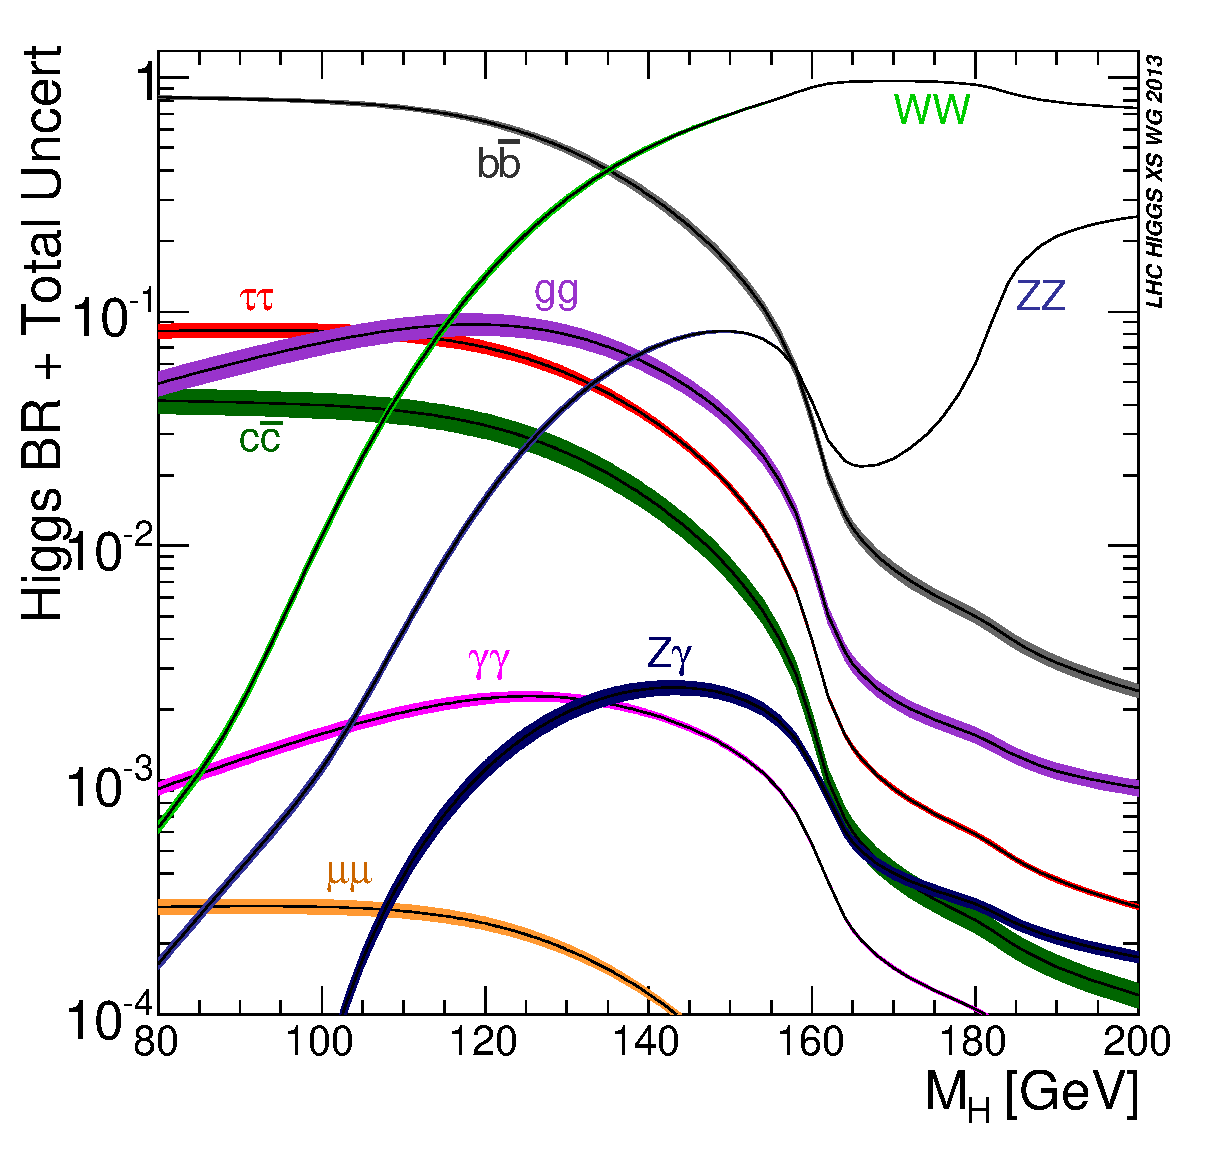
\includegraphics[width=0.5\linewidth]{T/FIGS/Higgs_BR_LM}
			\caption[Branching ratios of Higgs decay channels as a function of Higgs mass]{Higgs decay branching ratios with their uncertainties for the low mass region plotted as a function of Higgs mass \cite{LHCHiggsXS2013}.}
			\label{fig:higgsbrlm}
		\end{figure}

		At a Higgs mass of $\sim125$GeV the dominant decay mode is shown in Figure \ref{fig:higgsbrlm} to be the $H\rightarrow b\bar{b}$ mode. While this is the dominant decay mode at this Higgs mass, Higgs searches will make use of other decay channels where the final state signature is clearer and easier to trigger events on, such as the leptonic decays $H\rightarrow\tau\tau$ and $H\rightarrow\gamma\gamma$. Higgs decays to gauge bosons also offer clear final states as they will subsequently decay to leptons \cite{higgssearch}.

		At the LHC, the two main search channels for the Higgs boson are the \ggF\ production mode decaying to a $WW$ pair leading to a $l\nu l\nu$ final state \cite{hprod, searchggf} and the Higgs-Strahlung VH production with subsequent $H\rightarrow b\bar{b}$ and the vector boson $V$ ($V = W, Z$) decaying $V\rightarrow l+X$ \cite{hprod, searchvh}. The other principal production modes and alternative decay channels are also used in searches for the Higgs boson however. Searches in the $t\bar{t}H$ channel make use of the $t$ quarks decaying into one or zero leptons \cite{tth}, and vector boson fusion can exploit the distinctive final state signature. Discussion of VBF searches, specifically \VBFHBB, are given in Section \ref{t:VBF}.

	\subsection{Summary of Current Higgs Measurements}

		At the current point in time, the LHC has delivered more than $40$fb$^{-1}$ of $13$TeV $pp$ collisions to the ATLAS and CMS detectors (Section \ref{d:lhc}, and Higgs searches have been carried out in wide variety of decay channels ($WW$, $BB$, $\gamma\gamma$) and production modes (\ggF, VH, VBF) \cite{pdghiggs, VBFHbb8tev, searchggf, searchvh, tth}. Currently, the consensus of these analyses is that the CMS and ATLAS experiments have observed the Standard Model Higgs boson with a mass of $125.09\pm0.24$GeV\cite{pdg}.

	\subsection{Searches for \VBFHBB}
		\label{t:VBF}

		Production of a Higgs boson from the fusion of vector bosons radiated from initial-state quarks is the second largest cross-section at the LHC, and is useful as a production mode due to topological characteristics which can distinguish the event from \ggF. In \VBFHBB, the characteristic topology is a pair of central \bjets\ forming the Higgs candidate, and two forward, close to the beam line VBF jets formed from remnants of the initially colliding protons as displayed in Figure \ref{fig:higgsproddiag}. In addition, central jet activity is suppressed due to the lack of colour exchange between the colour singlet Higgs boson and the decay \bquarks\cite{VBF2004}.  These distinctive
		 features mean that VBF can be distinguished from the other production mechanisms.

		Searches for the \VBFHBB\, interaction look for a resonance in the invariant mass of a pair of jets containing \bquarks ($m_{bb}$) in events with the characteristic topology. This characteristic topology distinguishes the signal events from the multijet events that form the dominant background with a non-resonant $m_{bb}$ spectrum. An additional resonant background contribution to the \mbb spectrum is due to decay of a $Z$ boson to two jets in association with two jets \cite{VBFHbb8tev}. With the application of specific cuts to take advantage of this topology, the VBF channel provides a clean environment for analysis \cite{pdghiggs}.

		In the most recent searches for the Higgs boson produced via VBF, which this analysis emulates \cite{VBFHbb8tev}, the \VBFHBB\, events are separated from non-Higgs backgrounds using a multivariate boosted decision tree (BDT) analysis (Appendix \ref{a:bdt}) to refine the phase space to the most VBF sensitive BDT regions.


\endinput
